\chapter{Non-Key Attribute Organizations}
Other important organizations are the ones to retrieve records of a table that satisfy a query which involves nonkey attributes, i.e. attributes that do not uniquely identify a record.

\section{Non-Key Attribute Search}
The records to retrieve are specified with search conditions of the following types:
\begin{itemize}
    \item An \textit{equality search} which specifies a value \(v\) for an attribute \(Ai (Ai = vi)\)
    \item A \textit{range search}, which specifies a range of values for an attribute \(A_i (v_1 \leq A_i \leq v_2)\)
    \item A \textit{boolean search}, which consists of the previous search types combined with the operators AND, OR and NOT
\end{itemize}

\begin{figure}[!h]
    \centering
    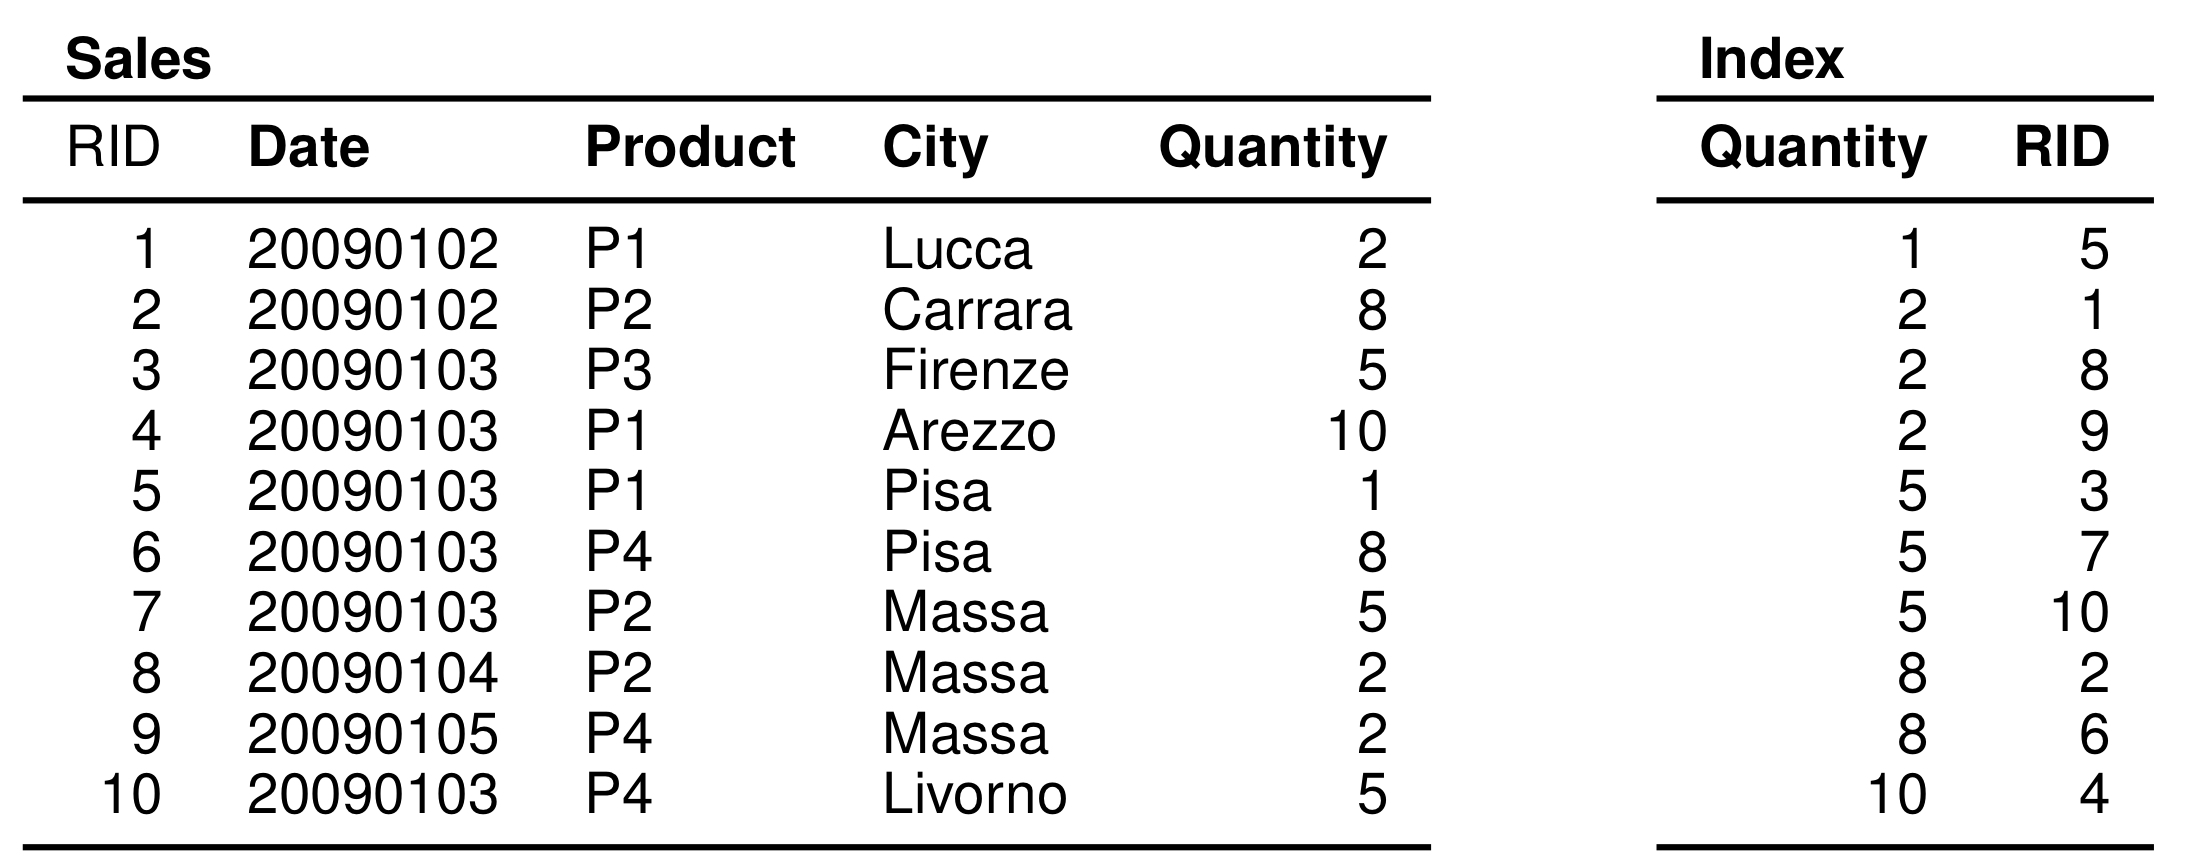
\includegraphics[width=0.7\linewidth]{images/DBMS_Internals/NonKeyAttributeOrganizations/index_on_quantity.jpeg}
    \caption{An Index on Quantity}
\end{figure}

New have the following proprieties:
\begin{itemize}
    \item With a primary organization, queries on non-key attributes can only be answered with a scan of the data. With large collections of records and queries satisfied by small subsets, if the response time is an important requirement, this approach is not worthwhile.
    \item Indexes are non-exclusive. Therefore they can be created for any non-key attributes, regardless of the primary organization used to store the table records.
    \item An excessive number of indexes can be harmful to the overall performance
    \item A typical implementation of an index is the inverted index organization
\end{itemize}


\section{Inverted Indexes}
\begin{tcolorbox}
An inverted index \(I\) on a non-key attribute \(K\) of a table \(R\) is a sorted collection of entries of the form \((k_i,n,p_1,p_2,...,p_n)\) where:
\begin{itemize}
    \item \(k_i\) is a specific value if \(K\)
    \item \(n\) is the number of records containing that value
    \item \(p_1,p_2,...,p_n\) is the \textit{sorted} RID list of these records
\end{itemize}
\end{tcolorbox}

\begin{figure}[!h]
    \centering
    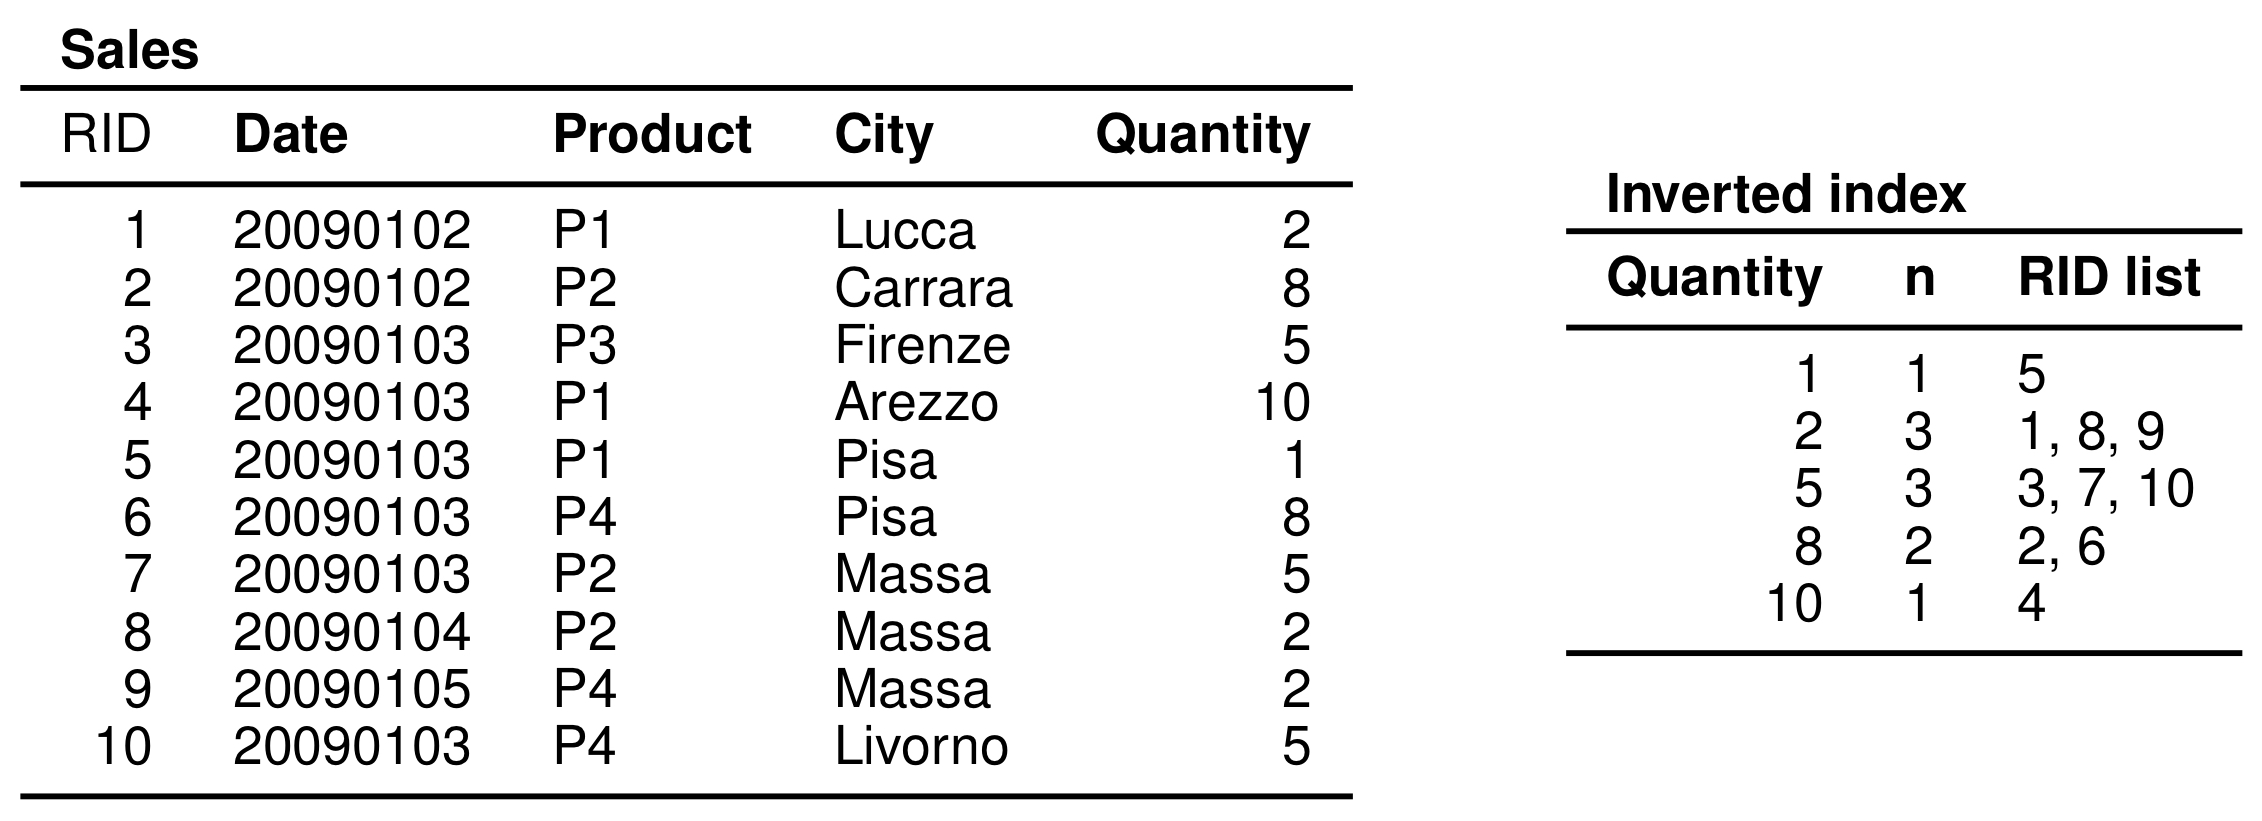
\includegraphics[width=0.7\linewidth]{images/DBMS_Internals/NonKeyAttributeOrganizations/inverted_index.jpeg}
    \caption{An \textit{inverted index} on Quantity}
\end{figure}

The advantage of using an \textbf{inverted index} are the following:
\begin{itemize}
    \item The data file is accessed only to find the records that match the query
    \item The result of “count” with conditions, or selection of index attributes can be satisfied with the use of only the index
    \item The organization of the file is independent from the organization of the index
\end{itemize}

\subsection{Performance Evaluation - (NOT REQUIRED)}
The performance is evaluated in terms of:
\begin{itemize}
    \item The amount of extra memory needed, not counting the memory needed to store the data file
    \item Cost of the search for records with specified values for the indexed attributes, and of the update operations
\end{itemize}

\subsubsection{Memory requirements}
\[
M = \text{Index memory}\]\[
\quad = \sum_{i=1}^{N_i(R)} N_{key}(I_i)(L_{I_i} + L_R) + N_I(R) \times N_{rec}(R) \times L_{RID}\]\[
\quad \approx N_I(R) \times N_{rec}(R) \times L_{RID}
\]

\subsection{Equality Search - (NOT REQUIRED)}
\[C_s = C_I + C_D\]
Where:
\begin{itemize}
    \item \(C_s\) is the cost of accessing the index pages
    \item \(C_D\) is the cost of accessing the data pages containing the records
\end{itemize}
The \textbf{selectivity factor} is determined by the multiplicity of keys
\[sf(cond) = sf(A_i = v_i) = \frac{1}{N_{key}(A_i)}\]
\(C_I\) is usually approximated to the cost of accessing the leaf nodes, ignoring the cost of the visit of the path from the root to a leaf node
\[C_I = \lceil sf(p) \times N_{leaf}(I)\rceil = \Bigg\lceil \frac{N_{leaf}(I)}{N_{key}(I)} \Bigg\rceil\]

\subsubsection{Unclustered Index}
If the index is \textbf{unclustered} it is necessary to have an estimate of the number of records \(E_{rec}\) satisfying the query condition \((A_i = v_i)\)
\[E_{rec} = \lceil sf(p) \times N_{rec}(R)\rceil = \Bigg\lceil \frac{N_{rec}(R)}{N_{key}(I)} \Bigg\rceil\]
The following formula is used to estimate \(C_D\):
\[C_D = \lceil \Phi(E_{rec}, N_{pag}(R) \rceil\]
\begin{tcolorbox}
Where the \(\Phi(k, n)\) is an estimate of the number of pages, in a file of n pages, that contain at least one of the k records to be retrieved using a \textit{sorted} rid-list. The following approximation is proposed by Cardenas:
\[
\Phi(k, n) = n \Bigg(1-\Bigg(1-\frac{1}{n}\Bigg)^k\Bigg)
\]
\[\Phi(k, n) \leq \min(k, n)\]
\end{tcolorbox}

\begin{figure}[!h]
    \centering
    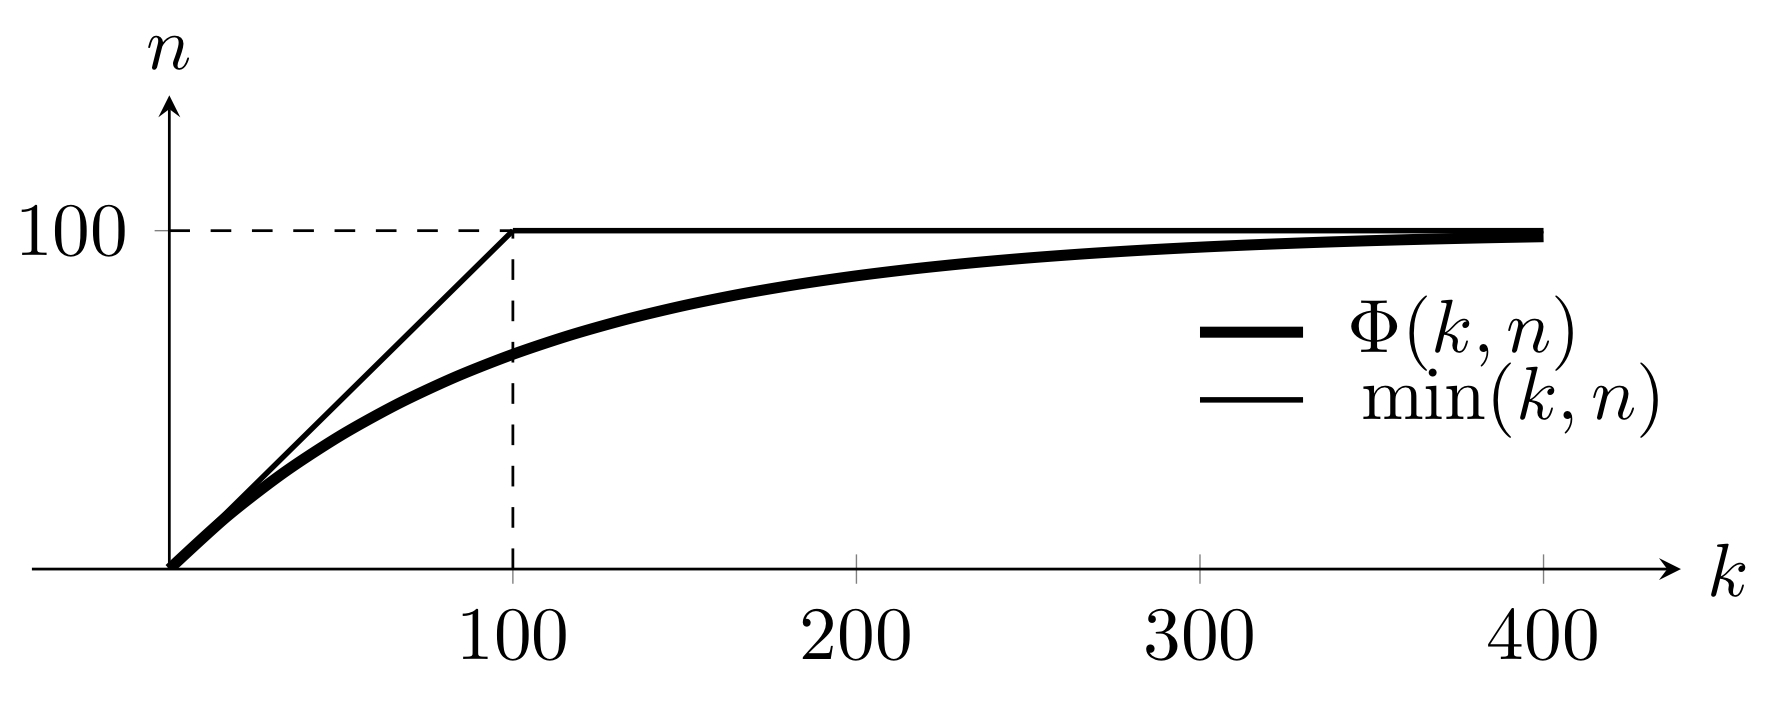
\includegraphics[width=0.5\linewidth]{images/DBMS_Internals/NonKeyAttributeOrganizations/phi_function.jpeg}
    \caption{Shape of \(\Phi\) function}
\end{figure}

\subsubsection{Clustered Index}
If the index is \textbf{clustered}, otherwise we have:
\[C_D = \lceil sf(p) \times N_{pag}(R)\rceil = \Bigg\lceil \frac{N_{pag}(R)}{N_{key}(I)} \Bigg\rceil\]


\subsection{Range Search - (NOT REQUIRED)}
Let us assume that to retrieve the records that satisfy the condition \(v_1 \leq A_i \leq v_2\), an equality search operation is performed for each \(Ai\) value in the range. The cost is:
\[C_s = C_I + C_D\]
Where
\begin{itemize}
    \item \(C_I = \lceil sf(p) \times N_{leaf}(I) \rceil\)
    \item \[sf(p) = \frac{v_2 - v_1}{\max(A_i) - \min(A_i)} \quad v_1 \leq A_i \leq v_2\]
    \item \(C_D = NoIndexKeyValues \times NoPageAccessesForRidList\)
    \item \(NoIndexKeyValues = \lceil sf(p) \times N_{key}(I) \rceil\)
    \item \(NoPageAccessesForRidList\) depends on the index type:
    \begin{itemize}
        \item \textbf{Clustered} \[C_D = \lceil sf(p) \times N_{pag}(R)\rceil = \Bigg\lceil \frac{N_{pag}(R)}{N_{key}(I)} \Bigg\rceil\]
        \item \textbf{Unclustered with ordered lists of RID} \[C_D = \Bigg\lceil \Phi\Bigg( \frac{N_{rec}(R)}{N_{key}(A_i)}, N_{pag}(R) \Bigg) \Bigg\rceil\]
    \end{itemize}
\end{itemize}

\section{Bitmap indexes}
\begin{tcolorbox}
A bitmap index \(I\) on a non-key attribute \(K\) of a table \(R\), with \(N\) records, is a sorted collection of entries of the form \((k_i, B)\), where each values \(k_i\) of \(K\) is followed by a sequence of N bits, where the \(j\)-th bit is set to 1 if the record \(j\)-th has the value \(k_i\) for the attribute \(K\). All other bits of the bitmap B are set to 0.
\end{tcolorbox}

The advantages of Bitmap Index are the following one:
\begin{itemize}
    \item Useful when the attribute has a low selectivity 
    \item Efficient bit operations for set-oriented operators 
    \item Optimal for queries which count the data
\end{itemize}

\begin{figure}[!h]
    \centering
    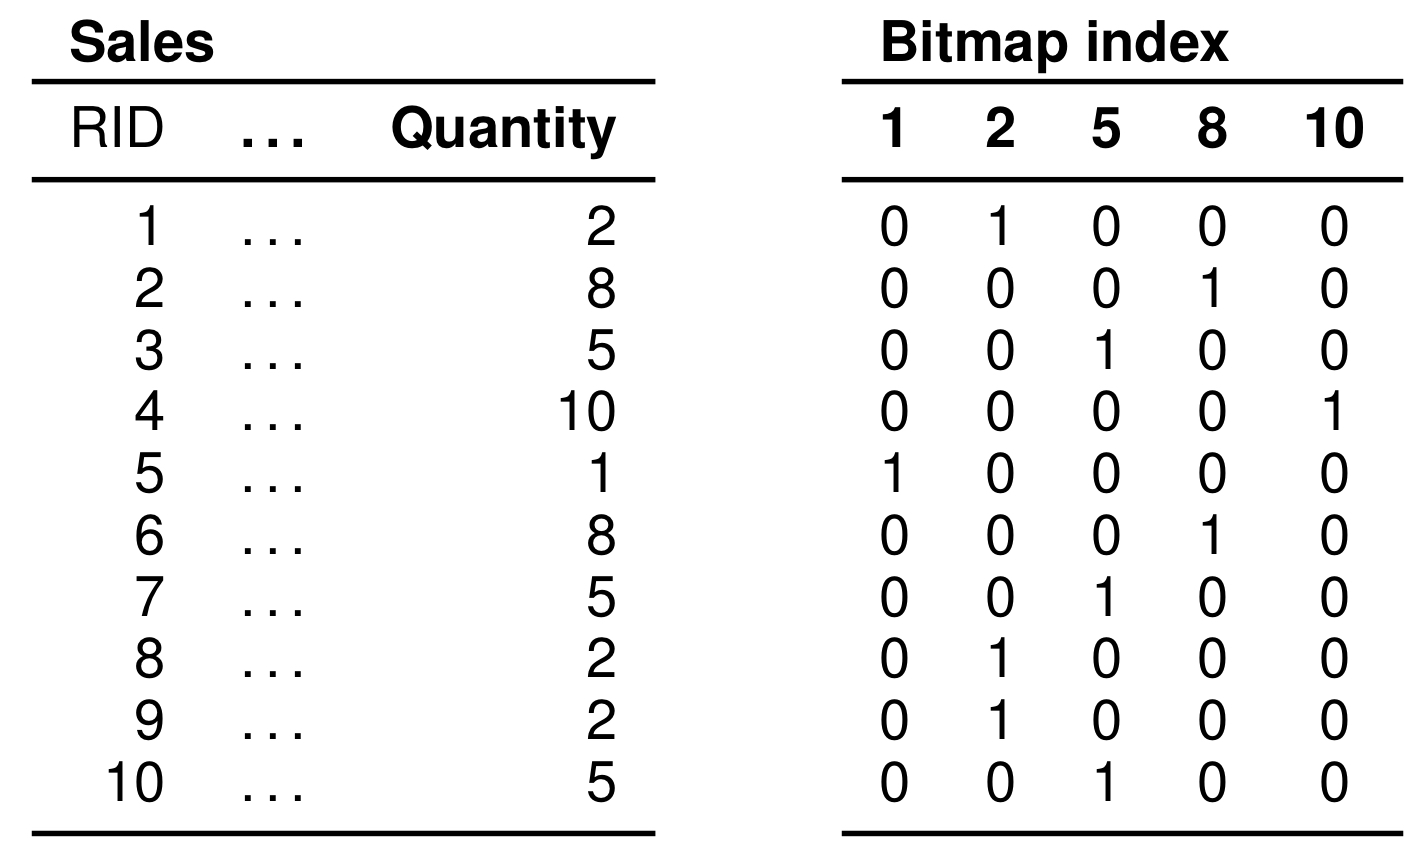
\includegraphics[width=0.5\linewidth]{images/DBMS_Internals/NonKeyAttributeOrganizations/bitmap_index.jpeg}
    \caption{A \textit{bitmap index} on Quantity}
\end{figure}

\subsection{Comparison with traditional indexes - (NOT REQUIRED)}
The number of \textbf{leaves} of an \textbf{inverted index} is:
\[N_{leaf} = \frac{(N_{key}) \times L_k + N_{rec} \times L_{RID}}{D_{pag}} \approx \frac{N_{rec} \times L_{RID}}{D_{pag}}\]
The number of \textbf{leaves} of a \textbf{bitmap index} is:
\[N_{leaf} = \frac{(N_{key}) \times L_k + N_{key} \times \frac{N_{rec}}{8}}{D_{pag}} \approx N_{key} \times \frac{N_{rec}}{D_{pag} \times 8}\]

\begin{figure}[!h]
    \centering
    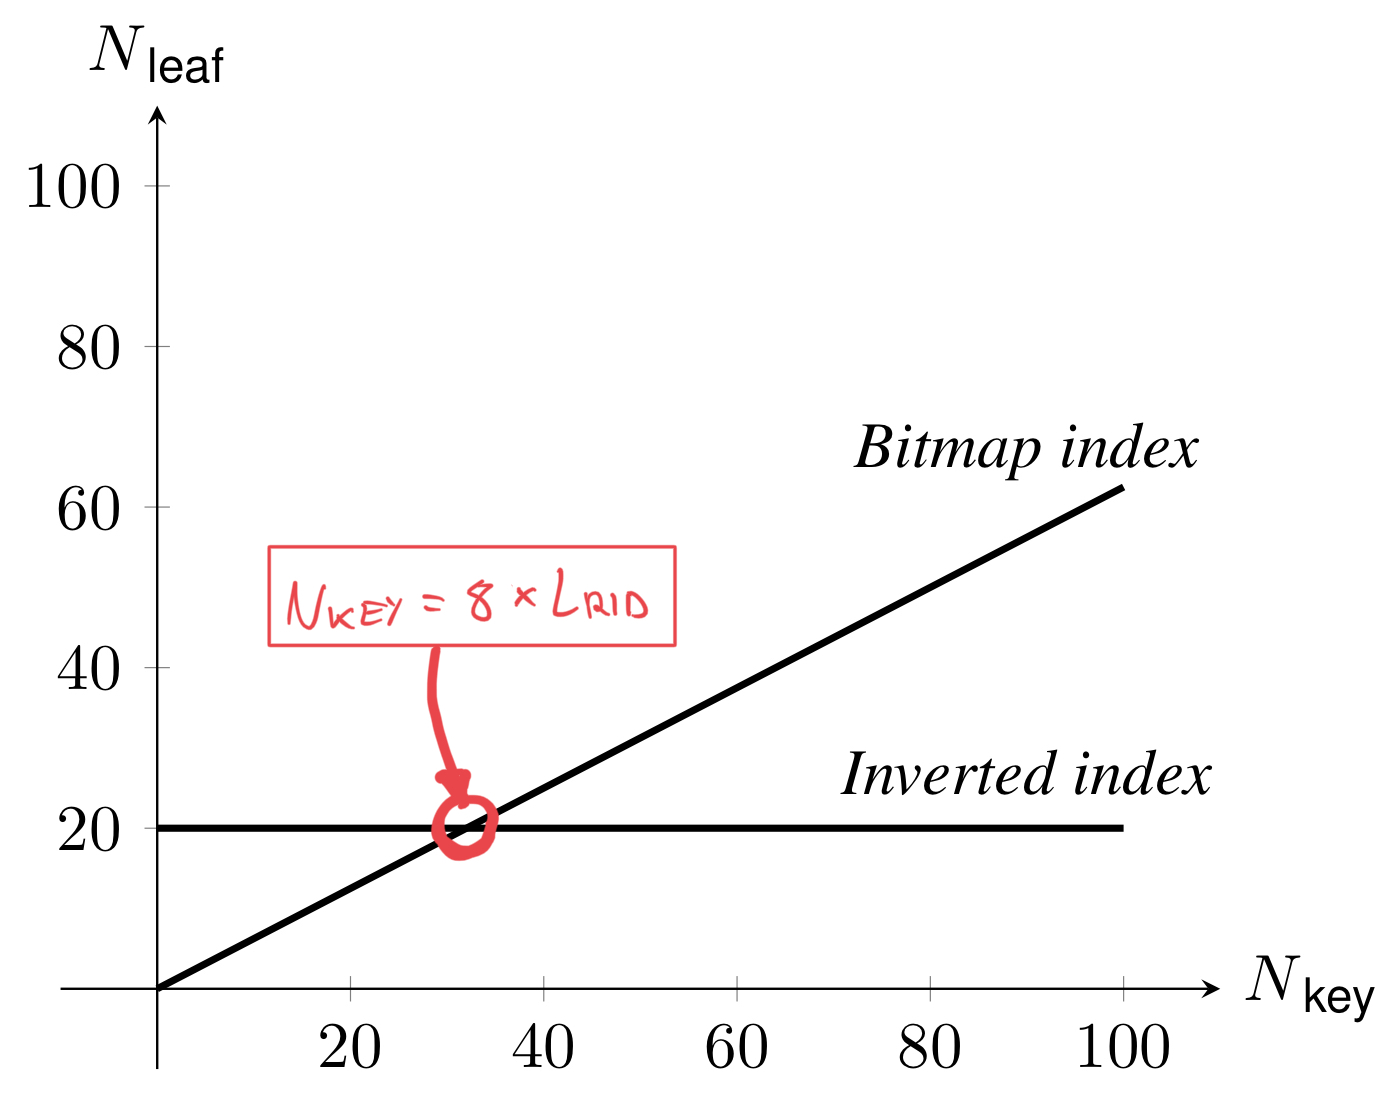
\includegraphics[width=0.45\linewidth]{images/DBMS_Internals/NonKeyAttributeOrganizations/indexes_comparison.jpeg}
\end{figure}

\section{Multi-attribute Index}
Let us see how to use inverted indexes to speed up the search of records that satisfy a conjunction of equality or range conditions on a subset of k attributes \(A_1, A_2,..., A_k\).

A query with a condition that uses all the k attributes is called \textit{exact match query}, otherwise is called \textit{partial match query}.

Let \(R(A_1, A_2, A_3)\) be a relation with \(N_{rec}(R)\) records. The attributes \(A_1, A_2, A_3\) have \(n_1, n_2\) and \(n_3\) distinct values. Three inverted indexes on each attribute have \((n_1+n_2+n_3)\) elements, and the total number of RIDs is \(3 \times N_{rec}(R)\).

An alternative solution to speed up the search consists in building a \textbf{multi-attribute (composite) index} on \(A_1, A_2, A_3\), with \((n1 \times n2 \times n3)\) elements, one for each combination of the values of the attributes \(A_i\), with the rid-lists of the records that have those three values in the three attributes. The total number of RIDs is now \(N_{rec}(R)\).